% -----------------------------------------------------------------------------
\documentclass[a4paper]{artikel3}
% -----------------------------------------------------------------------------
\paperheight = 29.70 cm  \paperwidth = 21.0 cm  \hoffset        = 0.46 cm
\headheight  =  0.81 cm  \textwidth  = 15.0 cm  \evensidemargin = 0.00 cm
\headsep     =  0.81 cm	 \textheight = 9.00 in  \oddsidemargin  = 0.00 cm					
% -----------------------------------------------------------------------------
\usepackage{enumerate}
\usepackage{amsfonts}
\usepackage{amsmath}
\usepackage{url}
\usepackage{graphicx}
\usepackage{float}
\usepackage[font=small,labelfont=bf]{caption}
\usepackage{setspace}
\usepackage{booktabs}
\usepackage[pdfpagemode=None,
		    colorlinks=true, 
		    urlcolor=blue,
		    linkcolor=blue, 
		    citecolor=blue, 
		    pdfstartview=FitH]{hyperref}
% -----------------------------------------------------------------------------
\newtheorem{thm}{Theorem}
\newtheorem{cor}[thm]{Corollary}
\newtheorem{lem}{Lemma}
\newtheorem{prop}{Proposition}
\newtheorem{definition}[thm]{Definition}
\newtheorem{rem}[thm]{Remark}
\newtheorem{exm}[thm]{Example}
% -----------------------------------------------------------------------------
\allowdisplaybreaks
\onehalfspacing
% -----------------------------------------------------------------------------
\begin{document}

% Title page
\begin{center}
{\Large \onehalfspacing \bf Comparing Unconstrained Optimization Methods}
\end{center}
\vspace{10pt}

\begin{center}
Jaan Tollander de Balsch\\
{\textit{{\small{Aalto University School of Science, Department of Computer Science, 
                \{de.tollander@aalto.fi\}}}}}
\end{center}

% \tableofcontents

\section{Project description}

\begin{table}[H]
\caption{Computer Details}
\label{tbl:1}
\centering
\begin{tabular}{l r r r}
\toprule
Detail & Value\\
\midrule
Operating System & Ubuntu 16.04 LTS \\
Memory (RAM) & 16 GiB \\
Processor & Inter Core i5-7600K CPU @ 3.80GHz $\times$ 4 \\
\bottomrule
\end{tabular}
\end{table}



\section{Numerical results}

\begin{figure}[H]
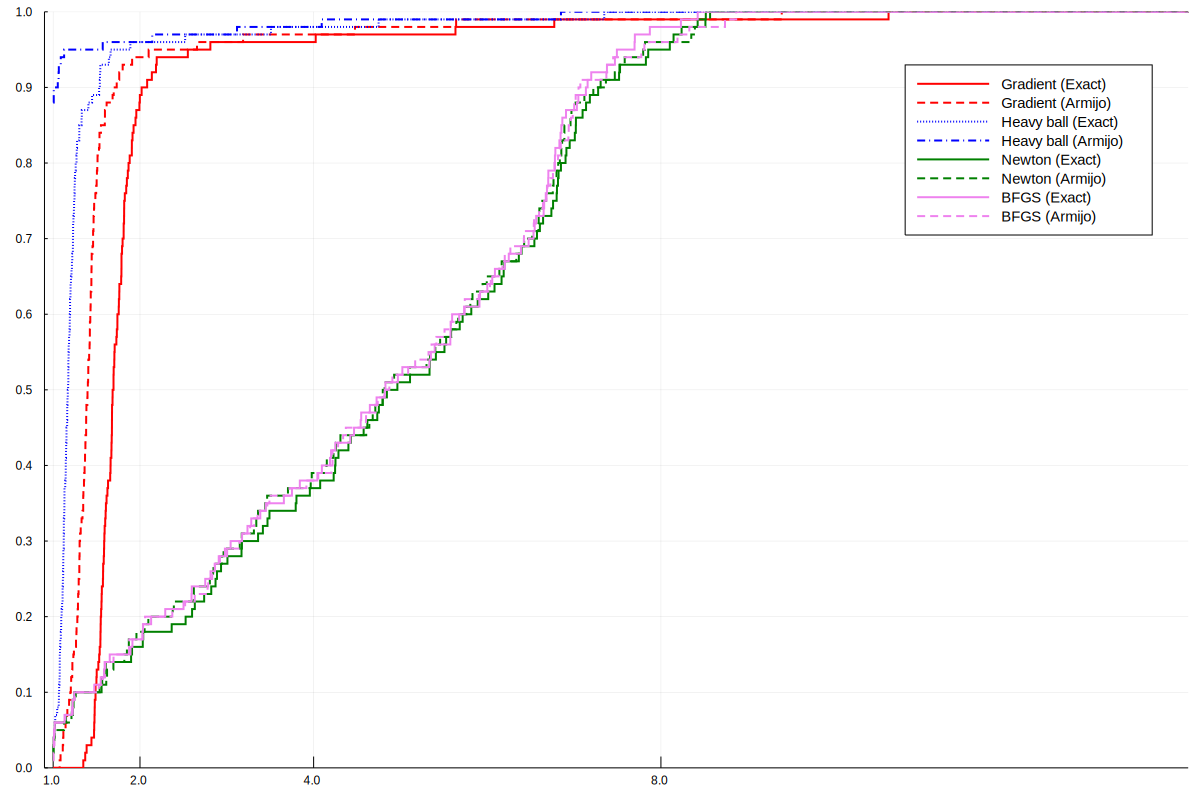
\includegraphics[scale=0.32]{figures/performance_plot_1.pdf}
\end{figure}


\begin{figure}[H]
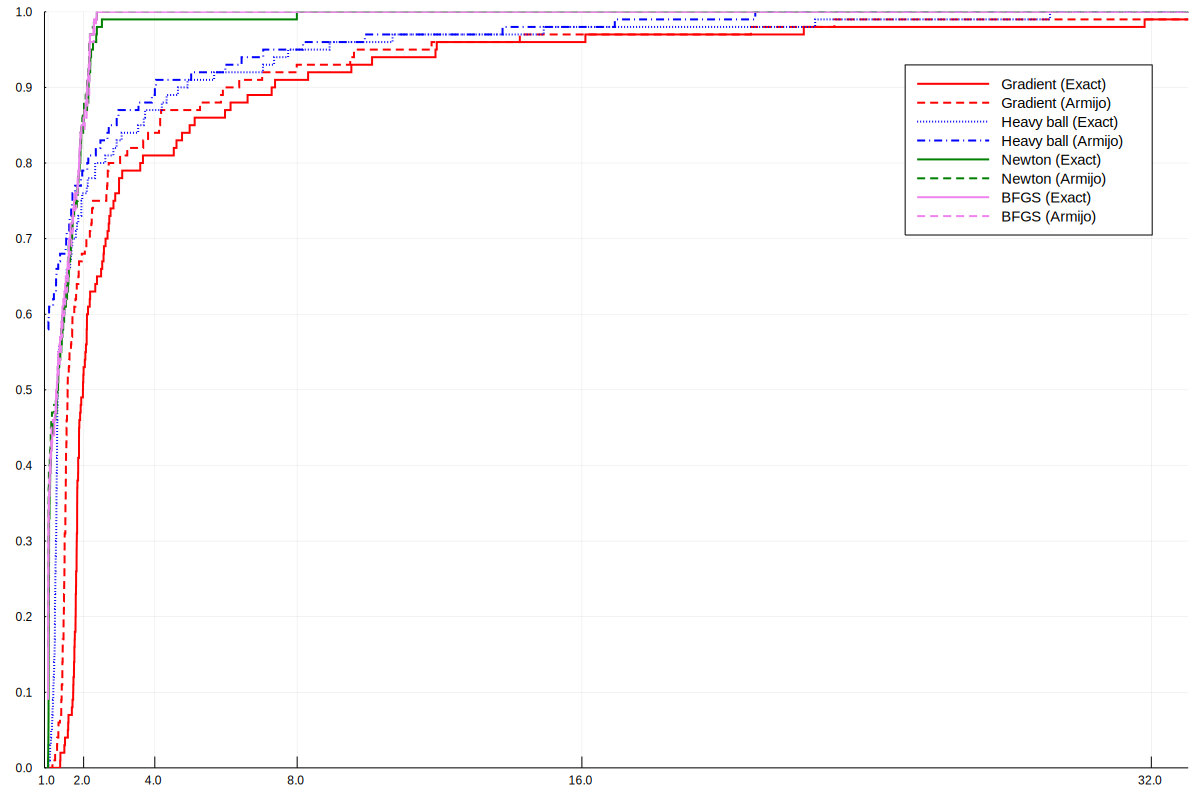
\includegraphics[scale=0.32]{figures/performance_plot_2.pdf}
\end{figure}


\section{Discussion and conclusions}



\end{document} 